\documentclass{article}

\usepackage[utf8]{inputenc}
\usepackage[letterpaper, total={6in, 9in}]{geometry}
\usepackage{amsmath}
\usepackage{natbib}
\usepackage{wrapfig}
\usepackage{graphicx}
\usepackage{amssymb}
\usepackage{tikz}

\graphicspath{ {./geo2/} }


\title{Geometry 2 - Circles}
\author{TSS Math Club}
\date{Oct 2022}

\begin{document}
\large

\maketitle

\section{Basic property of Circles}
\subsection{Definition of Circles}
\subsection{Terms to describe geometric object related to circles}
\begin{wrapfigure}{R}{0.4\textwidth} %this figure will be at the right
    \centering
    
    
    \tikzset{every picture/.style={line width=0.75pt}} %set default line width to 0.75pt        
    
    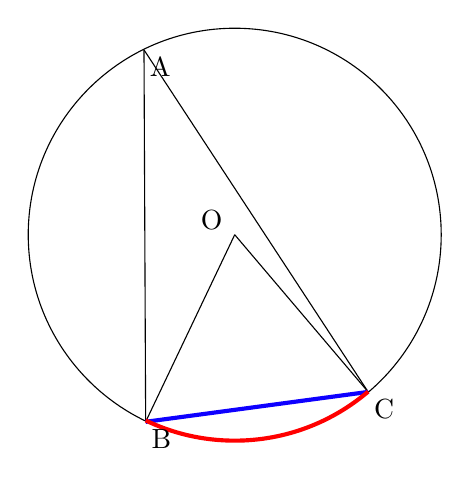
\begin{tikzpicture}[x=0.75pt,y=0.75pt,yscale=-0.8,xscale=0.8]
        %uncomment if require: \path (0,300); %set diagram left start at 0, and has height of 300
        
        %Shape: Circle [id:dp17379134999161217] 
        \draw   (28,148.36) .. controls (28,79.68) and (83.68,24) .. (152.36,24) .. controls (221.04,24) and (276.72,79.68) .. (276.72,148.36) .. controls (276.72,217.04) and (221.04,272.72) .. (152.36,272.72) .. controls (83.68,272.72) and (28,217.04) .. (28,148.36) -- cycle ;
        %Straight Lines [id:da45878936702265327] 
        \draw    (152.36,148.36) -- (232.72,243.03) ;
        %Straight Lines [id:da6953334630723775] 
        \draw    (152.36,148.36) -- (98.72,261.03) ;
        %Straight Lines [id:da21878844711573953] 
        \draw    (97.72,37.03) -- (98.72,261.03) ;
        %Straight Lines [id:da3182172562914929] 
        \draw    (97.72,37.03) -- (232.72,243.03) ;
        %Straight Lines [id:da9967812564105096] 
        \draw [color={rgb, 255:red, 14; green, 0; blue, 255 }  ,draw opacity=1 ][line width=1.5]    (98.72,261.03) -- (232.72,243.03) ;
        %Shape: Arc [id:dp9816832896319678] 
        \draw  [draw opacity=0][line width=1.5]  (232.73,242.82) .. controls (211.08,261.25) and (183.02,272.38) .. (152.36,272.38) .. controls (133.15,272.38) and (114.96,268.01) .. (98.72,260.21) -- (152.36,148.36) -- cycle ; \draw  [color={rgb, 255:red, 255; green, 0; blue, 0 }  ,draw opacity=1 ][line width=1.5]  (232.73,242.82) .. controls (211.08,261.25) and (183.02,272.38) .. (152.36,272.38) .. controls (133.15,272.38) and (114.96,268.01) .. (98.72,260.21) ;  
        
        % Text Node
        \draw (130.36,132.36) node [anchor=north west][inner sep=0.75pt]   [align=left] {O};
        % Text Node
        \draw (99.72,40.03) node [anchor=north west][inner sep=0.75pt]   [align=left] {A};
        % Text Node
        \draw (100.72,264.03) node [anchor=north west][inner sep=0.75pt]   [align=left] {B};
        % Text Node
        \draw (234.72,246.03) node [anchor=north west][inner sep=0.75pt]   [align=left] {C};
        
        
    \end{tikzpicture}
\end{wrapfigure}
Center: \\ \\
Radius: \\ \\
Arc: \\ \\
Chord: \\ \\
Central angle: \\ \\
Inscribed angle: \\ \\


\subsection{Central angle is twice any inscribed angle}




\tikzset{every picture/.style={line width=0.75pt}} %set default line width to 0.75pt        

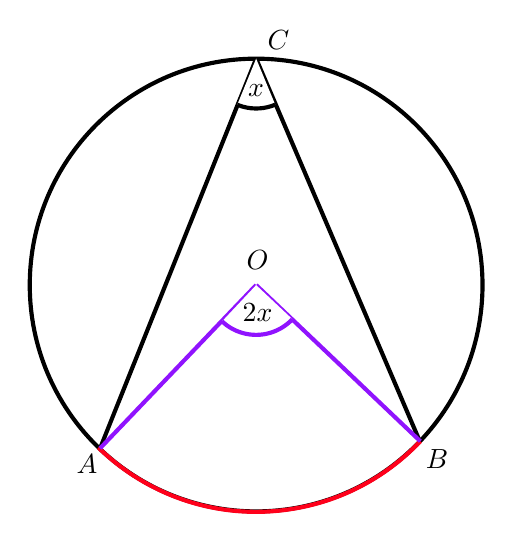
\begin{tikzpicture}[x=0.75pt,y=0.75pt,yscale=-0.8,xscale=0.8]
%uncomment if require: \path (0,419); %set diagram left start at 0, and has height of 419

%Shape: Circle [id:dp5403186956911956] 
\draw  [line width=1.5]  (203.33,174.67) .. controls (203.33,99.37) and (264.37,38.33) .. (339.67,38.33) .. controls (414.96,38.33) and (476,99.37) .. (476,174.67) .. controls (476,249.96) and (414.96,311) .. (339.67,311) .. controls (264.37,311) and (203.33,249.96) .. (203.33,174.67) -- cycle ;
%Straight Lines [id:da5957136609895495] 
\draw [color={rgb, 255:red, 0; green, 0; blue, 0 }  ,draw opacity=1 ][fill={rgb, 255:red, 255; green, 255; blue, 255 }  ,fill opacity=1 ][line width=1.5]    (339.67,38.33) -- (438.33,269) ;
%Straight Lines [id:da6339312134822053] 
\draw [color={rgb, 255:red, 0; green, 0; blue, 0 }  ,draw opacity=1 ][fill={rgb, 255:red, 255; green, 255; blue, 255 }  ,fill opacity=1 ][line width=1.5]    (339.67,38.33) -- (245.67,273) ;
%Shape: Arc [id:dp5366702840230211] 
\draw  [draw opacity=0][fill={rgb, 255:red, 255; green, 255; blue, 255 }  ,fill opacity=1 ][line width=1.5]  (351.17,66.04) .. controls (345.14,68.55) and (338.25,69.12) .. (331.48,67.2) .. controls (330.39,66.88) and (329.32,66.52) .. (328.29,66.09) -- (339.67,38.33) -- cycle ; \draw  [color={rgb, 255:red, 0; green, 0; blue, 0 }  ,draw opacity=1 ][line width=1.5]  (351.17,66.04) .. controls (345.14,68.55) and (338.25,69.12) .. (331.48,67.2) .. controls (330.39,66.88) and (329.32,66.52) .. (328.29,66.09) ;  
%Shape: Arc [id:dp9498591182227187] 
\draw  [draw opacity=0][line width=1.5]  (438.55,268.73) .. controls (417.51,290.96) and (388.92,306.26) .. (356.19,310.24) .. controls (313.61,315.44) and (273.22,300.36) .. (244.66,272.57) -- (339.67,174.67) -- cycle ; \draw  [color={rgb, 255:red, 255; green, 0; blue, 27 }  ,draw opacity=1 ][line width=1.5]  (438.55,268.73) .. controls (417.51,290.96) and (388.92,306.26) .. (356.19,310.24) .. controls (313.61,315.44) and (273.22,300.36) .. (244.66,272.57) ;  
%Straight Lines [id:da06768614777660997] 
\draw [color={rgb, 255:red, 144; green, 19; blue, 254 }  ,draw opacity=1 ][line width=1.5]    (339.67,174.67) -- (245.67,273) ;
%Straight Lines [id:da712391157904465] 
\draw [color={rgb, 255:red, 144; green, 19; blue, 254 }  ,draw opacity=1 ][line width=1.5]    (339.67,174.67) -- (438.55,268.73) ;
%Shape: Arc [id:dp1573251124672308] 
\draw  [draw opacity=0][fill={rgb, 255:red, 255; green, 255; blue, 255 }  ,fill opacity=1 ][line width=1.5]  (361.51,195.24) .. controls (354.08,203.12) and (342.62,206.69) .. (331.48,203.53) .. controls (326.7,202.17) and (322.52,199.73) .. (319.14,196.55) -- (339.67,174.67) -- cycle ; \draw  [color={rgb, 255:red, 144; green, 19; blue, 254 }  ,draw opacity=1 ][line width=1.5]  (361.51,195.24) .. controls (354.08,203.12) and (342.62,206.69) .. (331.48,203.53) .. controls (326.7,202.17) and (322.52,199.73) .. (319.14,196.55) ;  

% Text Node
\draw (333.33,52.07) node [anchor=north west][inner sep=0.75pt]    {$x$};
% Text Node
\draw (230,275.4) node [anchor=north west][inner sep=0.75pt]    {$A$};
% Text Node
\draw (440.33,272.4) node [anchor=north west][inner sep=0.75pt]    {$B$};
% Text Node
\draw (330,184.4) node [anchor=north west][inner sep=0.75pt]    {$2x$};
% Text Node
\draw (332.33,152.07) node [anchor=north west][inner sep=0.75pt]    {$O$};
% Text Node
\draw (345,20) node [anchor=north west][inner sep=0.75pt]    {$C$};

\end{tikzpicture}



\pagebreak

\subsection{Inscribed angles subtended by the same arc are equal}



\tikzset{every picture/.style={line width=0.75pt}} %set default line width to 0.75pt        

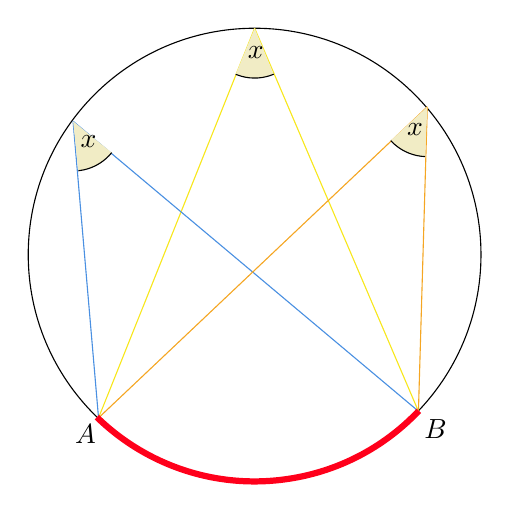
\begin{tikzpicture}[x=0.75pt,y=0.75pt,yscale=-0.8,xscale=0.8]
%uncomment if require: \path (0,419); %set diagram left start at 0, and has height of 419

%Shape: Circle [id:dp5403186956911956] 
\draw   (203.33,174.67) .. controls (203.33,99.37) and (264.37,38.33) .. (339.67,38.33) .. controls (414.96,38.33) and (476,99.37) .. (476,174.67) .. controls (476,249.96) and (414.96,311) .. (339.67,311) .. controls (264.37,311) and (203.33,249.96) .. (203.33,174.67) -- cycle ;
%Straight Lines [id:da5957136609895495] 
\draw [color={rgb, 255:red, 248; green, 231; blue, 28 }  ,draw opacity=1 ][fill={rgb, 255:red, 241; green, 236; blue, 197 }  ,fill opacity=1 ]   (339.67,38.33) -- (438.33,269) ;
%Straight Lines [id:da33122143131158555] 
\draw [color={rgb, 255:red, 74; green, 144; blue, 226 }  ,draw opacity=1 ][fill={rgb, 255:red, 241; green, 236; blue, 197 }  ,fill opacity=1 ]   (230.33,94.33) -- (245.67,273) ;
%Straight Lines [id:da6339312134822053] 
\draw [color={rgb, 255:red, 248; green, 231; blue, 28 }  ,draw opacity=1 ][fill={rgb, 255:red, 241; green, 236; blue, 197 }  ,fill opacity=1 ]   (339.67,38.33) -- (245.67,273) ;
%Straight Lines [id:da8938383138384509] 
\draw [color={rgb, 255:red, 74; green, 144; blue, 226 }  ,draw opacity=1 ][fill={rgb, 255:red, 241; green, 236; blue, 197 }  ,fill opacity=1 ]   (230.33,94.33) -- (267.33,125.4) -- (438.33,269) ;
%Straight Lines [id:da24326554605856554] 
\draw [color={rgb, 255:red, 245; green, 166; blue, 35 }  ,draw opacity=1 ][fill={rgb, 255:red, 241; green, 236; blue, 197 }  ,fill opacity=1 ]   (245.67,273) -- (443.67,85.67) ;
%Straight Lines [id:da9944164254362617] 
\draw [color={rgb, 255:red, 245; green, 166; blue, 35 }  ,draw opacity=1 ][fill={rgb, 255:red, 241; green, 236; blue, 197 }  ,fill opacity=1 ]   (443.67,85.67) -- (438.33,269) ;
%Shape: Arc [id:dp2640858128507122] 
\draw  [draw opacity=0][fill={rgb, 255:red, 241; green, 236; blue, 197 }  ,fill opacity=1 ] (253.62,113.25) .. controls (249.5,118.32) and (243.71,122.09) .. (236.84,123.62) .. controls (235.73,123.87) and (234.61,124.05) .. (233.51,124.17) -- (230.33,94.33) -- cycle ; \draw   (253.62,113.25) .. controls (249.5,118.32) and (243.71,122.09) .. (236.84,123.62) .. controls (235.73,123.87) and (234.61,124.05) .. (233.51,124.17) ;  
%Shape: Arc [id:dp5366702840230211] 
\draw  [draw opacity=0][fill={rgb, 255:red, 241; green, 236; blue, 197 }  ,fill opacity=1 ] (351.17,66.04) .. controls (345.14,68.55) and (338.25,69.12) .. (331.48,67.2) .. controls (330.39,66.88) and (329.32,66.52) .. (328.29,66.09) -- (339.67,38.33) -- cycle ; \draw   (351.17,66.04) .. controls (345.14,68.55) and (338.25,69.12) .. (331.48,67.2) .. controls (330.39,66.88) and (329.32,66.52) .. (328.29,66.09) ;  
%Shape: Arc [id:dp5386457051908322] 
\draw  [draw opacity=0][fill={rgb, 255:red, 241; green, 236; blue, 197 }  ,fill opacity=1 ] (442.39,115.64) .. controls (435.86,115.37) and (429.38,112.97) .. (424.06,108.37) .. controls (423.19,107.62) and (422.38,106.84) .. (421.62,106.02) -- (443.67,85.67) -- cycle ; \draw   (442.39,115.64) .. controls (435.86,115.37) and (429.38,112.97) .. (424.06,108.37) .. controls (423.19,107.62) and (422.38,106.84) .. (421.62,106.02) ;  
%Shape: Arc [id:dp9498591182227187] 
\draw  [draw opacity=0][line width=2.25]  (438.55,268.73) .. controls (417.51,290.96) and (388.92,306.26) .. (356.19,310.24) .. controls (313.61,315.44) and (273.22,300.36) .. (244.66,272.57) -- (339.67,174.67) -- cycle ; \draw  [color={rgb, 255:red, 255; green, 0; blue, 27 }  ,draw opacity=1 ][line width=2.25]  (438.55,268.73) .. controls (417.51,290.96) and (388.92,306.26) .. (356.19,310.24) .. controls (313.61,315.44) and (273.22,300.36) .. (244.66,272.57) ;  

% Text Node
\draw (233.33,101.4) node [anchor=north west][inner sep=0.75pt]    {$x$};
% Text Node
\draw (334,48.07) node [anchor=north west][inner sep=0.75pt]    {$x$};
% Text Node
\draw (430,94.07) node [anchor=north west][inner sep=0.75pt]    {$x$};
% Text Node
\draw (230,275.4) node [anchor=north west][inner sep=0.75pt]    {$A$};
% Text Node
\draw (440.33,272.4) node [anchor=north west][inner sep=0.75pt]    {$B$};

\end{tikzpicture}


\vspace{40px}

\subsection{Angle subtended by a diameter is \(90^{\circ}\)}


\tikzset{every picture/.style={line width=0.75pt}} %set default line width to 0.75pt        

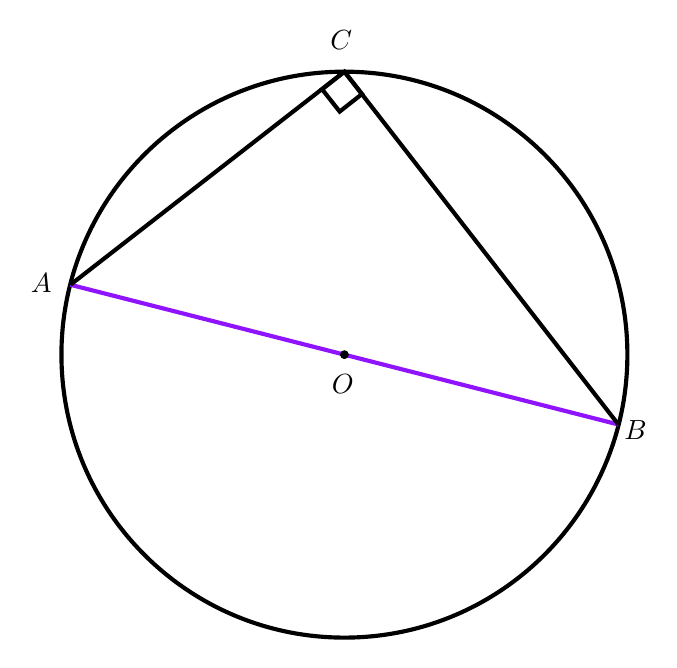
\begin{tikzpicture}[x=0.75pt,y=0.75pt,yscale=-1,xscale=1]
%uncomment if require: \path (0,419); %set diagram left start at 0, and has height of 419

%Shape: Circle [id:dp5403186956911956] 
\draw  [line width=1.5]  (203.33,174.67) .. controls (203.33,99.37) and (264.37,38.33) .. (339.67,38.33) .. controls (414.96,38.33) and (476,99.37) .. (476,174.67) .. controls (476,249.96) and (414.96,311) .. (339.67,311) .. controls (264.37,311) and (203.33,249.96) .. (203.33,174.67) -- cycle ;
%Straight Lines [id:da06811875685737068] 
\draw [color={rgb, 255:red, 144; green, 19; blue, 254 }  ,draw opacity=1 ][line width=1.5]    (339.67,174.67) -- (471.67,208.33) ;
%Straight Lines [id:da4067465378250854] 
\draw [color={rgb, 255:red, 144; green, 19; blue, 254 }  ,draw opacity=1 ][line width=1.5]    (207.67,141) -- (339.67,174.67) ;
%Straight Lines [id:da6912410596897796] 
\draw [line width=1.5]    (339.67,38.33) -- (471.67,208.33) ;
%Straight Lines [id:da8601096491144575] 
\draw [line width=1.5]    (339.67,38.33) -- (207.67,141) ;
%Shape: Square [id:dp24268413759610286] 
\draw  [line width=1.5]  (328.91,46.8) -- (339.67,38.33) -- (348.14,49.09) -- (337.38,57.56) -- cycle ;
%Shape: Circle [id:dp8767343798761416] 
\draw  [fill={rgb, 255:red, 0; green, 0; blue, 0 }  ,fill opacity=1 ] (337.83,174.67) .. controls (337.83,173.65) and (338.65,172.83) .. (339.67,172.83) .. controls (340.68,172.83) and (341.5,173.65) .. (341.5,174.67) .. controls (341.5,175.68) and (340.68,176.5) .. (339.67,176.5) .. controls (338.65,176.5) and (337.83,175.68) .. (337.83,174.67) -- cycle ;

% Text Node
\draw (187.33,134.4) node [anchor=north west][inner sep=0.75pt]    {$A$};
% Text Node
\draw (473.33,205.07) node [anchor=north west][inner sep=0.75pt]    {$B$};
% Text Node
\draw (331.67,17.4) node [anchor=north west][inner sep=0.75pt]    {$C$};
% Text Node
\draw (332.33,183.07) node [anchor=north west][inner sep=0.75pt]    {$O$};


\end{tikzpicture}



\pagebreak

\subsection{Perpendicular chord theorem}



\tikzset{every picture/.style={line width=0.75pt}} %set default line width to 0.75pt        

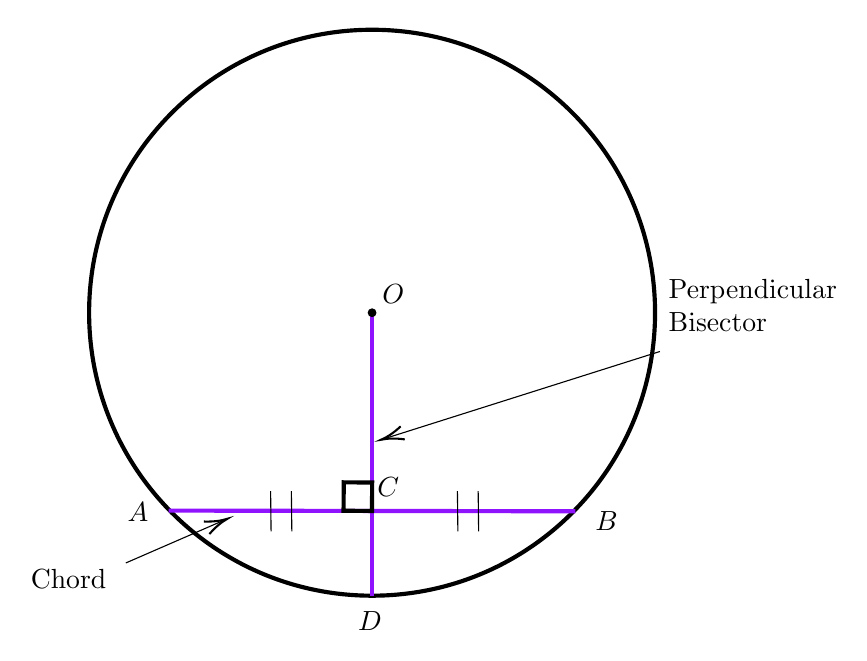
\begin{tikzpicture}[x=0.75pt,y=0.75pt,yscale=-1,xscale=1]
%uncomment if require: \path (0,419); %set diagram left start at 0, and has height of 419

%Shape: Circle [id:dp5403186956911956] 
\draw  [line width=1.5]  (203.33,174.67) .. controls (203.33,99.37) and (264.37,38.33) .. (339.67,38.33) .. controls (414.96,38.33) and (476,99.37) .. (476,174.67) .. controls (476,249.96) and (414.96,311) .. (339.67,311) .. controls (264.37,311) and (203.33,249.96) .. (203.33,174.67) -- cycle ;
%Straight Lines [id:da06811875685737068] 
\draw [color={rgb, 255:red, 144; green, 19; blue, 254 }  ,draw opacity=1 ][line width=1.5]    (241.67,270) -- (437.56,270.33) ;
%Straight Lines [id:da4067465378250854] 
\draw [color={rgb, 255:red, 144; green, 19; blue, 254 }  ,draw opacity=1 ][line width=1.5]    (339.67,311) -- (339.67,174.67) ;
%Shape: Circle [id:dp8767343798761416] 
\draw  [fill={rgb, 255:red, 0; green, 0; blue, 0 }  ,fill opacity=1 ] (337.83,174.67) .. controls (337.83,173.65) and (338.65,172.83) .. (339.67,172.83) .. controls (340.68,172.83) and (341.5,173.65) .. (341.5,174.67) .. controls (341.5,175.68) and (340.68,176.5) .. (339.67,176.5) .. controls (338.65,176.5) and (337.83,175.68) .. (337.83,174.67) -- cycle ;
%Shape: Square [id:dp7558142713797231] 
\draw  [line width=1.5]  (326.02,256.38) -- (339.71,256.48) -- (339.61,270.17) -- (325.92,270.07) -- cycle ;
%Straight Lines [id:da40971348906843996] 
\draw    (300.78,260.67) -- (301,280) ;
%Straight Lines [id:da8507674313612943] 
\draw    (290.78,260.67) -- (291,280) ;
%Straight Lines [id:da007449580833429614] 
\draw    (390.78,260.67) -- (391,280) ;
%Straight Lines [id:da4940931408813922] 
\draw    (380.78,260.67) -- (381,280) ;

% Text Node
\draw (481.33,157.22) node [anchor=north west][inner sep=0.75pt]   [align=left] {Perpendicular \\Bisector};
% Text Node
\draw (330,229.56) node [anchor=north west][inner sep=0.75pt]   [align=left] { };
% Text Node
\draw (174,297.11) node [anchor=north west][inner sep=0.75pt]   [align=left] {Chord};
% Text Node
\draw (273,261.22) node [anchor=north west][inner sep=0.75pt]   [align=left] { };
% Text Node
\draw (343.33,160.07) node [anchor=north west][inner sep=0.75pt]    {$O$};
% Text Node
\draw (220.67,264.96) node [anchor=north west][inner sep=0.75pt]    {$A$};
% Text Node
\draw (446,269.29) node [anchor=north west][inner sep=0.75pt]    {$B$};
% Text Node
\draw (341,252.62) node [anchor=north west][inner sep=0.75pt]    {$C$};
% Text Node
\draw (331.67,317.29) node [anchor=north west][inner sep=0.75pt]    {$D$};
% Connection
\draw    (478.33,193.34) -- (345.91,235.26) ;
\draw [shift={(344,235.86)}, rotate = 342.43] [color={rgb, 255:red, 0; green, 0; blue, 0 }  ][line width=0.75]    (10.93,-3.29) .. controls (6.95,-1.4) and (3.31,-0.3) .. (0,0) .. controls (3.31,0.3) and (6.95,1.4) .. (10.93,3.29)   ;
% Connection
\draw    (221,295.24) -- (268.17,274.72) ;
\draw [shift={(270,273.92)}, rotate = 156.49] [color={rgb, 255:red, 0; green, 0; blue, 0 }  ][line width=0.75]    (10.93,-3.29) .. controls (6.95,-1.4) and (3.31,-0.3) .. (0,0) .. controls (3.31,0.3) and (6.95,1.4) .. (10.93,3.29)   ;

\end{tikzpicture}


\vspace{50px}

\subsection{Tangent to a circle}

\subsubsection{Definition:}
\vspace{20px}

\subsubsection{The radius from the center of the circle to the point of tangency is perpendicular to the tangent line}



\tikzset{every picture/.style={line width=0.75pt}} %set default line width to 0.75pt        

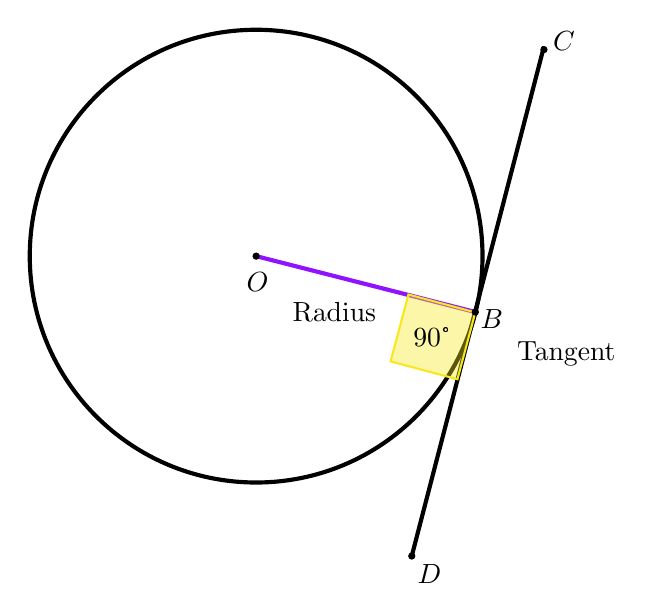
\begin{tikzpicture}[x=0.75pt,y=0.75pt,yscale=-0.8,xscale=0.8]
%uncomment if require: \path (0,419); %set diagram left start at 0, and has height of 419

%Shape: Circle [id:dp5403186956911956] 
\draw  [line width=1.5]  (203.33,174.67) .. controls (203.33,99.37) and (264.37,38.33) .. (339.67,38.33) .. controls (414.96,38.33) and (476,99.37) .. (476,174.67) .. controls (476,249.96) and (414.96,311) .. (339.67,311) .. controls (264.37,311) and (203.33,249.96) .. (203.33,174.67) -- cycle ;
%Straight Lines [id:da06811875685737068] 
\draw [color={rgb, 255:red, 144; green, 19; blue, 254 }  ,draw opacity=1 ][line width=1.5]    (339.67,174.67) -- (471.67,208.33) ;
%Shape: Circle [id:dp8767343798761416] 
\draw  [fill={rgb, 255:red, 0; green, 0; blue, 0 }  ,fill opacity=1 ] (337.83,174.67) .. controls (337.83,173.65) and (338.65,172.83) .. (339.67,172.83) .. controls (340.68,172.83) and (341.5,173.65) .. (341.5,174.67) .. controls (341.5,175.68) and (340.68,176.5) .. (339.67,176.5) .. controls (338.65,176.5) and (337.83,175.68) .. (337.83,174.67) -- cycle ;
%Straight Lines [id:da10641417010205423] 
\draw [line width=1.5]    (433.4,355.27) -- (513,48.47) ;
%Shape: Square [id:dp24268413759610286] 
\draw  [color={rgb, 255:red, 248; green, 231; blue, 28 }  ,draw opacity=1 ][fill={rgb, 255:red, 248; green, 231; blue, 28 }  ,fill opacity=0.38 ][line width=0.75]  (431.39,197.78) -- (471.67,208.53) -- (460.91,248.81) -- (420.64,238.06) -- cycle ;
%Shape: Circle [id:dp49749378737218897] 
\draw  [fill={rgb, 255:red, 0; green, 0; blue, 0 }  ,fill opacity=1 ] (469.83,208.33) .. controls (469.83,207.32) and (470.65,206.5) .. (471.67,206.5) .. controls (472.68,206.5) and (473.5,207.32) .. (473.5,208.33) .. controls (473.5,209.35) and (472.68,210.17) .. (471.67,210.17) .. controls (470.65,210.17) and (469.83,209.35) .. (469.83,208.33) -- cycle ;
%Shape: Circle [id:dp7955108597985465] 
\draw  [fill={rgb, 255:red, 0; green, 0; blue, 0 }  ,fill opacity=1 ] (431.57,355.27) .. controls (431.57,354.25) and (432.39,353.43) .. (433.4,353.43) .. controls (434.41,353.43) and (435.23,354.25) .. (435.23,355.27) .. controls (435.23,356.28) and (434.41,357.1) .. (433.4,357.1) .. controls (432.39,357.1) and (431.57,356.28) .. (431.57,355.27) -- cycle ;
%Shape: Circle [id:dp0003285569832827129] 
\draw  [fill={rgb, 255:red, 0; green, 0; blue, 0 }  ,fill opacity=1 ] (511.17,50.3) .. controls (511.17,49.29) and (511.99,48.47) .. (513,48.47) .. controls (514.01,48.47) and (514.83,49.29) .. (514.83,50.3) .. controls (514.83,51.31) and (514.01,52.13) .. (513,52.13) .. controls (511.99,52.13) and (511.17,51.31) .. (511.17,50.3) -- cycle ;

% Text Node
\draw (473.33,205.07) node [anchor=north west][inner sep=0.75pt]    {$B$};
% Text Node
\draw (517,37.87) node [anchor=north west][inner sep=0.75pt]    {$C$};
% Text Node
\draw (332.33,183.07) node [anchor=north west][inner sep=0.75pt]    {$O$};
% Text Node
\draw (435.4,358.67) node [anchor=north west][inner sep=0.75pt]    {$D$};
% Text Node
\draw (360,201.07) node [anchor=north west][inner sep=0.75pt]   [align=left] {Radius};
% Text Node
\draw (495.2,224.47) node [anchor=north west][inner sep=0.75pt]   [align=left] {Tangent};
% Text Node
\draw (432.8,216.07) node [anchor=north west][inner sep=0.75pt]   [align=left] {90°};


\end{tikzpicture}


\pagebreak

\subsubsection{The length of tangents from a point to a circle are equal}





\tikzset{every picture/.style={line width=0.75pt}} %set default line width to 0.75pt        

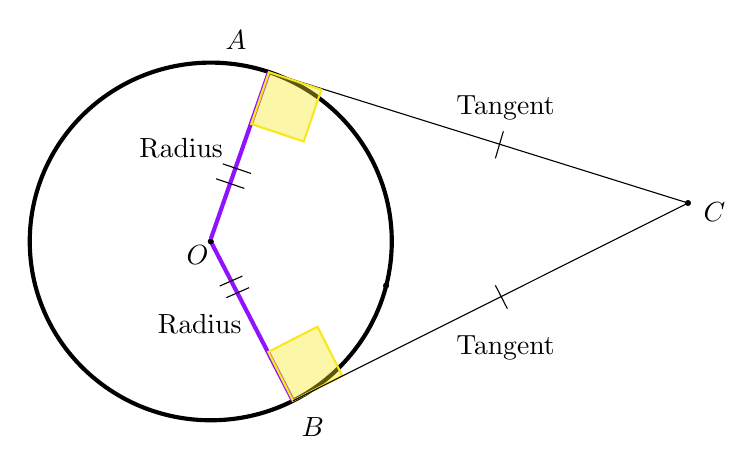
\begin{tikzpicture}[x=0.75pt,y=0.75pt,yscale=-0.8,xscale=0.8]
%uncomment if require: \path (0,419); %set diagram left start at 0, and has height of 419

%Shape: Ellipse [id:dp5403186956911956] 
\draw  [line width=1.5]  (121.97,174.07) .. controls (121.97,114.59) and (170.78,66.37) .. (230.99,66.37) .. controls (291.19,66.37) and (340,114.59) .. (340,174.07) .. controls (340,233.55) and (291.19,281.77) .. (230.99,281.77) .. controls (170.78,281.77) and (121.97,233.55) .. (121.97,174.07) -- cycle ;
%Straight Lines [id:da06811875685737068] 
\draw [color={rgb, 255:red, 144; green, 19; blue, 254 }  ,draw opacity=1 ][line width=1.5]    (230.99,174.07) -- (280.51,270.02) ;
%Shape: Ellipse [id:dp8767343798761416] 
\draw  [fill={rgb, 255:red, 0; green, 0; blue, 0 }  ,fill opacity=1 ] (229.52,174.07) .. controls (229.52,173.27) and (230.18,172.62) .. (230.99,172.62) .. controls (231.8,172.62) and (232.45,173.27) .. (232.45,174.07) .. controls (232.45,174.87) and (231.8,175.52) .. (230.99,175.52) .. controls (230.18,175.52) and (229.52,174.87) .. (229.52,174.07) -- cycle ;
%Shape: Ellipse [id:dp49749378737218897] 
\draw  [fill={rgb, 255:red, 0; green, 0; blue, 0 }  ,fill opacity=1 ] (335.07,200.67) .. controls (335.07,199.87) and (335.73,199.22) .. (336.54,199.22) .. controls (337.34,199.22) and (338,199.87) .. (338,200.67) .. controls (338,201.47) and (337.34,202.11) .. (336.54,202.11) .. controls (335.73,202.11) and (335.07,201.47) .. (335.07,200.67) -- cycle ;
%Straight Lines [id:da5760829311199731] 
\draw [color={rgb, 255:red, 144; green, 19; blue, 254 }  ,draw opacity=1 ][line width=1.5]    (266,72.13) -- (230.99,172.62) ;
%Straight Lines [id:da2529972826216105] 
\draw    (266,72.13) -- (518.4,150.93) ;
%Shape: Rectangle [id:dp2266551022394412] 
\draw  [color={rgb, 255:red, 248; green, 231; blue, 28 }  ,draw opacity=1 ][fill={rgb, 255:red, 248; green, 231; blue, 28 }  ,fill opacity=0.38 ][line width=0.75]  (265.62,240.62) -- (295.25,225.4) -- (310.13,254.81) -- (280.51,270.02) -- cycle ;
%Straight Lines [id:da9997015914374205] 
\draw    (280.51,270.02) -- (518.4,150.93) ;
%Shape: Ellipse [id:dp3407280289462833] 
\draw  [fill={rgb, 255:red, 0; green, 0; blue, 0 }  ,fill opacity=1 ] (516.93,150.93) .. controls (516.93,150.13) and (517.59,149.49) .. (518.4,149.49) .. controls (519.21,149.49) and (519.87,150.13) .. (519.87,150.93) .. controls (519.87,151.73) and (519.21,152.38) .. (518.4,152.38) .. controls (517.59,152.38) and (516.93,151.73) .. (516.93,150.93) -- cycle ;
%Straight Lines [id:da10566410471438958] 
\draw    (407.2,107.73) -- (402.4,124) ;
%Straight Lines [id:da6249154348250314] 
\draw    (402.4,200.53) -- (409.6,214.53) ;
%Straight Lines [id:da8015437869803181] 
\draw    (234.2,136.33) -- (251.2,142.13) ;
%Straight Lines [id:da2681549788104458] 
\draw    (236.4,200.93) -- (250,194.93) ;
%Straight Lines [id:da160461329674082] 
\draw    (240.4,207.93) -- (254,201.93) ;
%Straight Lines [id:da6992096843482827] 
\draw    (238.2,127.33) -- (255.2,133.13) ;
%Shape: Rectangle [id:dp24268413759610286] 
\draw  [color={rgb, 255:red, 248; green, 231; blue, 28 }  ,draw opacity=1 ][fill={rgb, 255:red, 248; green, 231; blue, 28 }  ,fill opacity=0.38 ][line width=0.75]  (266,72.13) -- (297.59,82.69) -- (286.96,113.88) -- (255.37,103.33) -- cycle ;

% Text Node
\draw (284.11,278.54) node [anchor=north west][inner sep=0.75pt]    {$B$};
% Text Node
\draw (526.2,148.91) node [anchor=north west][inner sep=0.75pt]    {$C$};
% Text Node
\draw (214.88,174.69) node [anchor=north west][inner sep=0.75pt]    {$O$};
% Text Node
\draw (197.56,216.1) node [anchor=north west][inner sep=0.75pt]   [align=left] {Radius};
% Text Node
\draw (377.28,229.32) node [anchor=north west][inner sep=0.75pt]   [align=left] {Tangent};
% Text Node
\draw (238.37,45.66) node [anchor=north west][inner sep=0.75pt]    {$A$};
% Text Node
\draw (186.36,110.5) node [anchor=north west][inner sep=0.75pt]   [align=left] {Radius};
% Text Node
\draw (377.28,84.52) node [anchor=north west][inner sep=0.75pt]   [align=left] {Tangent};


\end{tikzpicture}



\vspace{50px}

\subsubsection{Tangent-Chord Theorem: the angle formed between a chord and a tangent line to a circle is equal to the inscribed angle on the other side of the chord}



\tikzset{every picture/.style={line width=0.75pt}} %set default line width to 0.75pt        

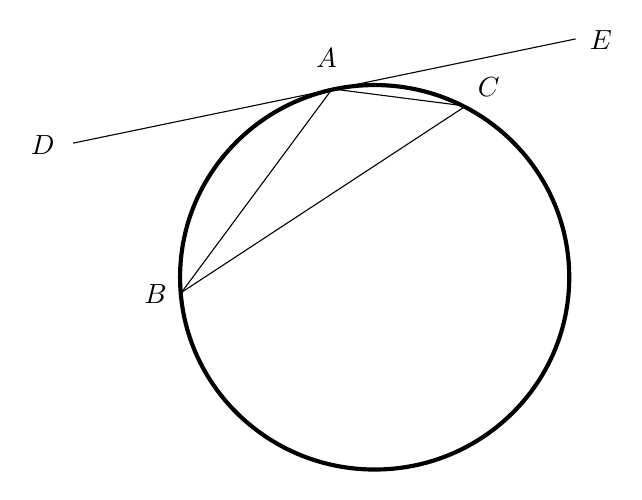
\begin{tikzpicture}[x=0.75pt,y=0.75pt,yscale=-0.86,xscale=0.86]
%uncomment if require: \path (0,419); %set diagram left start at 0, and has height of 419

%Shape: Ellipse [id:dp5403186956911956] 
\draw  [line width=1.5]  (158.37,284.87) .. controls (158.37,225.39) and (207.18,177.17) .. (267.39,177.17) .. controls (327.59,177.17) and (376.4,225.39) .. (376.4,284.87) .. controls (376.4,344.35) and (327.59,392.57) .. (267.39,392.57) .. controls (207.18,392.57) and (158.37,344.35) .. (158.37,284.87) -- cycle ;
%Straight Lines [id:da2529972826216105] 
\draw    (98.4,209.73) -- (380,151.33) ;
%Straight Lines [id:da24490325767999077] 
\draw    (243.6,179.33) -- (318.4,188.93) ;
%Straight Lines [id:da7066815250038527] 
\draw    (243.6,179.33) -- (159.2,293.33) ;
%Straight Lines [id:da354126616106069] 
\draw    (318.4,188.93) -- (159.2,293.33) ;

% Text Node
\draw (136.91,287.74) node [anchor=north west][inner sep=0.75pt]    {$B$};
% Text Node
\draw (323.8,171.71) node [anchor=north west][inner sep=0.75pt]    {$C$};
% Text Node
\draw (233.17,155.26) node [anchor=north west][inner sep=0.75pt]    {$A$};
% Text Node
\draw (73.31,204.14) node [anchor=north west][inner sep=0.75pt]    {$D$};
% Text Node
\draw (386.51,145.34) node [anchor=north west][inner sep=0.75pt]    {$E$};


\end{tikzpicture}


\pagebreak

\section{Cyclic Quadrilateral (Four points cyclic)}

\subsection{Definition}

\vspace{20px}

\subsection{Opposite angles are added up to \(180^{\circ}\)}

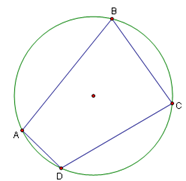
\includegraphics[scale=.8]{Picture9.png}

\subsection{How to prove four points cyclic}

\subsubsection{Prove these four points lies equally distance to another point — the center of the circle}

\subsubsection{Two equal angles subtend a segment (chord in the circle)}

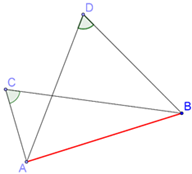
\includegraphics{Picture10.png}

\subsubsection{Opposite angles are added up to \(180^{\circ}\)}

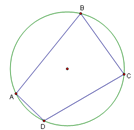
\includegraphics{Picture11.png}

\pagebreak

\section{Similar triangles involving a circle}

\subsection{Identify as many similar triangles as possible}

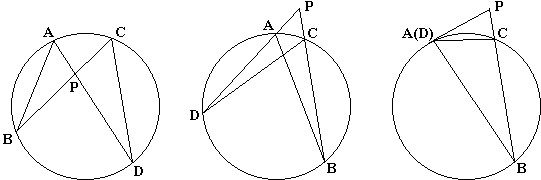
\includegraphics[scale=.75]{Picture12.jpg}

\vspace{100px}

\subsection{Power of a point}

\subsubsection{Definition:}

\vspace{20px}

\subsubsection{Power of point is fixed regardless the choice of chord}

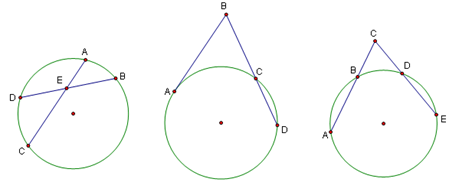
\includegraphics[scale=1.2]{Picture13.png}

\pagebreak

\subsubsection{Power of a point formula}

\[PoP = {PO}^2+r^2\]

\begin{center}
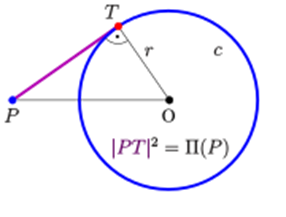
\includegraphics{Picture14.png}
\end{center}

\vspace{60px}

\subsection{Homothety involving circles}

\subsubsection{Homothety of a circle is a circle}

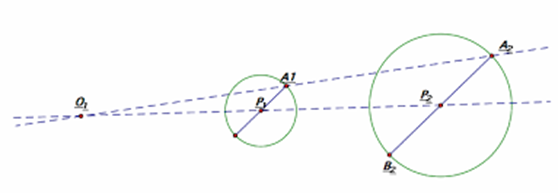
\includegraphics{Picture15.png}

\subsubsection{Ratios in the homothety}

\pagebreak

\section{Problems}

\subsection{Problem}
Given AD AE are the internal, external angle bisector of angle A,
 such that D,E are the intersection of the angle bisectors with the circumcircle. 
 Prove DE is a diameter of the circle.

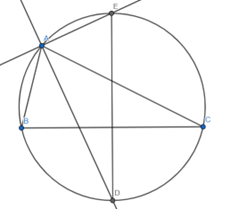
\includegraphics{Picture16.png}

\vspace{50px}

\subsection{Problem}
Given Circle C1, C2 intersect at A, B, CD is the common tangent to both circles, 
E is the intersection of AB and CD. Prove E is the midpoint of CD.

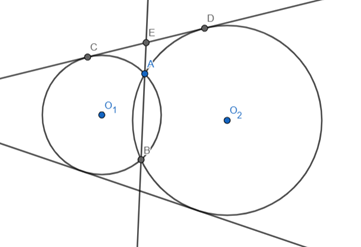
\includegraphics{Picture17.png}

\pagebreak

\subsection{Theorem}
In a triangle abc=4RS

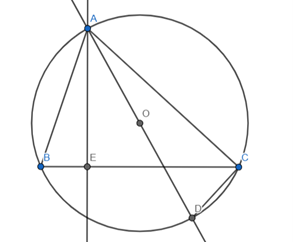
\includegraphics{Picture18.png}

\pagebreak

\subsection{Problem}

Given AE is the external angle bisector of angle A, 
AE intersects BC at G, 
the tangent at A intersects BC at F. 
Prove AFG is an isosceles triangle.

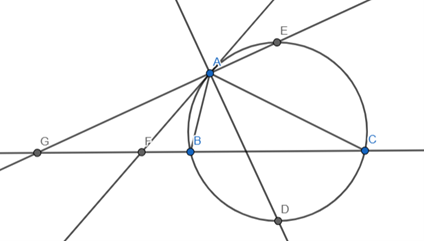
\includegraphics{Picture19.png}

\pagebreak

\subsection{Ptolemy's theorem}

If a quadrilateral is inscribed in a circle then the product of the lengths of its diagonals is equal to the sum of the products of the lengths of the pairs of opposite sides.
\\Or ab+cd=xy where a,b,c,d are the sides of the quadrilateral and x,y are the diagonals.

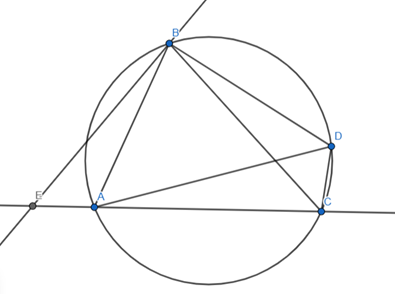
\includegraphics{Picture20.png}

\pagebreak

\subsection{Problem}
In \(\triangle\)ABC, point D is inside of ABC such that \(\angle \mathrm{DAC} = \angle \mathrm{DCA}=30^{\circ} \) and \(\angle \mathrm{DBA}=60^{\circ}\). E is the midpoint on BC and F is a trisect point on AC such that \(\mathrm{CF} = \frac{\mathrm{CA}}{3} \). Prove DE \(\perp\) EF.

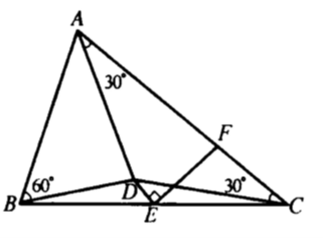
\includegraphics{Picture21.png}

\end{document}
